
% =============================================================================
\input{resources/preamble.tex}
% ============================================================================ 
\begin{document}
\onecolumn

% step {{{

\begin{figure}[h!]

\pgfplotsset{compat=newest} 
\pgfplotsset{soldot/.style={color=red,only marks,mark=*}}
\pgfplotsset{holdot/.style={color=red,fill=white,only marks,thick,mark=*}}

\begin{tikzpicture}
\begin{axis}[
title = STEP,
axis lines = left,
legend pos = outer north east,
xlabel = $x$,
ylabel = {$\sigma(x)$},
]
%Below the red parabola is defined
\addplot[domain=-10:0,red,ultra thick] {0};
\addplot[domain=0:10,red,ultra thick] {1};
\draw[dotted, red] (axis cs:0,0) -- (axis cs:0,1);
\addplot[holdot] coordinates{(0,0)};
\addplot[soldot] coordinates{(0,1)};
\end{axis}
\end{tikzpicture}

\caption{}
\label{fig:placeholder}
\end{figure}
% }}}
% sigmoid {{{

\begin{figure}[h!]

\begin{tikzpicture}
\definecolor{my_orange}{RGB}{255,102,0} 
\begin{axis}[
title = SIGMOID,
axis lines = center,
legend pos = outer north east,
xlabel = $x$,
ylabel = {$\sigma(x)$},
]
%Below the red parabola is defined
\addplot [
samples=100,
color=my_orange,
ultra thick,
]
{ 1/(1+exp(-x))};
\addlegendentry{$\sigma(x) = \frac{1}{1+e^{-x}}$}
\end{axis}
\end{tikzpicture}


\caption{}
\label{fig:placeholder}
\end{figure}
% }}}
% hyperbolic tangent {{{

\begin{figure}[h!]
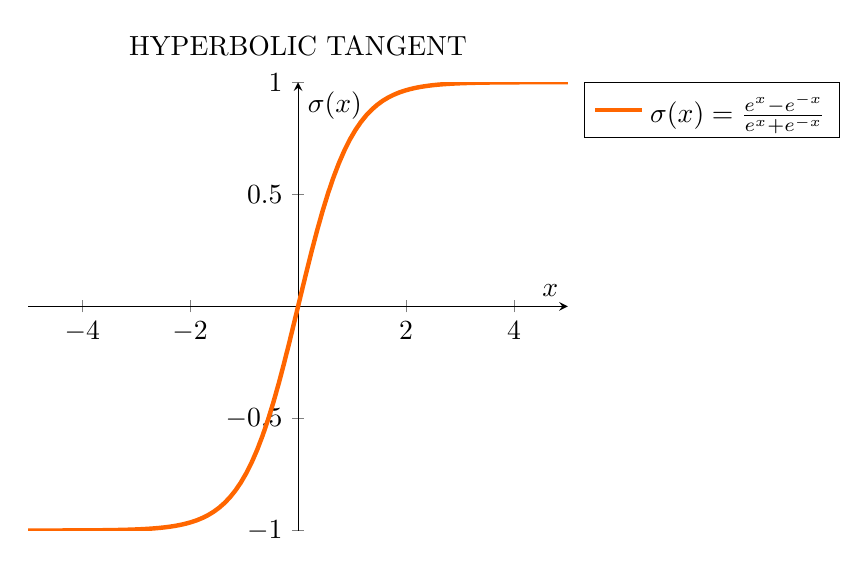
\begin{tikzpicture}
\definecolor{my_orange}{RGB}{255,102,0}
\begin{axis}[
title = HYPERBOLIC TANGENT,
axis lines = center,
legend pos = outer north east,
xlabel = $x$,
ylabel = {$\sigma(x)$},
]
%Below the red parabola is defined
\addplot [
samples=100,
color=my_orange,
ultra thick
]
{ (exp(x)-exp(-x))/(exp(x)+exp(-x))};
\addlegendentry{$\sigma(x) = \frac{e^x-e^{-x}}{e^x+e^{-x}}$}

\end{axis}
\end{tikzpicture}


\caption{}
\label{fig:placeholder}
\end{figure}
% }}}

% tkiz two column {{{

\begin{figure}[h!]
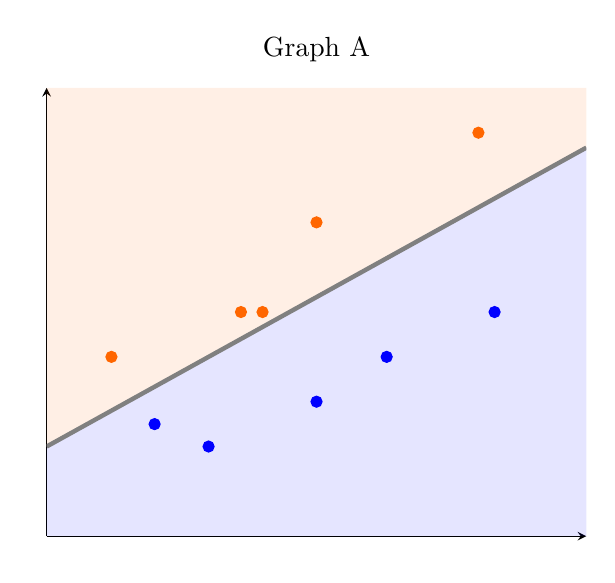
\begin{tikzpicture}

\usepgfplotslibrary{fillbetween}
\pgfplotsset{compat=newest}
\definecolor{my_orange}{RGB}{255,102,0}
\pgfplotsset{soldot/.style={color=my_orange,only marks,mark=*}}
\pgfplotsset{blue_soldot/.style={color=blue,only marks,mark=*}}
\pgfplotsset{ignore zero/.style={%
#1ticklabel={\ifdim\tick pt=0pt \else\pgfmathprintnumber{\tick}\fi}
}}


\begin{axis}[
title = Graph A,
axis lines = left,
axis line style={black},
every axis label/.append style ={black},
every tick label/.append style={black},
legend pos = outer north east,
xlabel = $$,
ylabel = $$,
ticks=none,
xmin=0,ymin=0,domain=0:10,ignore zero=x
]

% Draw random scatter of training data
\addplot[soldot] coordinates{(1.2,4)};
\addplot[blue_soldot] coordinates{(2,2.5)};
\addplot[blue_soldot] coordinates{(3,2)};
\addplot[soldot] coordinates{(3.6,5)};
\addplot[blue_soldot] coordinates{(5,3)};
\addplot[soldot] coordinates{(5,7)};
\addplot[soldot] coordinates{(4,5)};
\addplot[blue_soldot] coordinates{(6.3,4)};
\addplot[soldot] coordinates{(8,9)};
\addplot[blue_soldot] coordinates{(8.3,5)};

% Draw best fit example line
\addplot [
samples=100,
color=gray,
ultra thick,
name path=A
]
{ (x/1.5)+2 };

\addplot+[draw=none,mark=none,name path=B] {0}; % “fictional” curve
\addplot+[draw=none,mark=none,name path=C] {10}; % “fictional” curve
\addplot+[blue,opacity=0.1] fill between[of=A and B,soft clip={domain=0:10}]; % filling
\addplot+[my_orange,opacity=0.1] fill between[of=C and A,soft clip={domain=0:10}]; % filling

\end{axis}
\end{tikzpicture}


\caption{}
\label{fig:placeholder}
\end{figure}
% }}}
% tkiz two column {{{

\begin{figure}[h!]

\begin{tikzpicture}

\definecolor{my_orange}{RGB}{255,102,0}
\pgfplotsset{soldot/.style={color=my_orange,only marks,mark=*}}
\pgfplotsset{blue_soldot/.style={color=blue,only marks,mark=*}}
\pgfplotsset{ignore zero/.style={%
#1ticklabel={\ifdim\tick pt=0pt \else\pgfmathprintnumber{\tick}\fi}
}}

\begin{axis}[
title = Graph B,
axis lines = left,
axis line style={black},
every axis label/.append style ={black},
every tick label/.append style={black},
legend pos = outer north east,
xlabel = $$,
ylabel = $$,
ticks=none,
xmin=0,ymin=0,ymax=8,domain=0:10,ignore zero=x,
]
%\hspace{8cm}

% Draw random scatter of training data
\addplot[blue_soldot] coordinates{(1.2,4)};
\addplot[blue_soldot] coordinates{(2,2.5)};
\addplot[blue_soldot] coordinates{(4.8,1.5)};
\addplot[blue_soldot] coordinates{(4.2,2)};
\addplot[blue_soldot] coordinates{(5,0.8)};
\addplot[blue_soldot] coordinates{(6.3,1.7)};
\addplot[blue_soldot] coordinates{(3,2)};

\addplot[soldot] coordinates{(3.6,3.8)};
\addplot[soldot] coordinates{(3.53,3.5)};
\addplot[soldot] coordinates{(3,5)};
\addplot[soldot] coordinates{(4,5)};
\addplot[soldot] coordinates{(5,7)};
\addplot[soldot] coordinates{(8,9)};
\addplot[soldot] coordinates{(8.3,5)};

% Draw best fit example line
\addplot [
samples=100,
color=gray,
ultra thick,
domain=0:10,
name path=A
]
{{0.25*(x-5)^2 + 2}};

\addplot+[draw=none,mark=none,name path=B,domain=0:10] {0}; ; % “fictional” curve
\addplot+[blue,opacity=0.1] fill between[of=A and B,soft clip={domain=0:10}]; % filling

\addplot+[draw=none,mark=none,name path=C,domain=0:10] {8}; ; % “fictional” curve
\addplot+[my_orange,opacity=0.1] fill between[of=C and A,soft clip={domain=0:10}]; % filling

\end{axis}
\end{tikzpicture}

\caption{}
\label{fig:placeholder}
\end{figure}
% }}}
% tkiz two column {{{

\begin{figure}[h!]
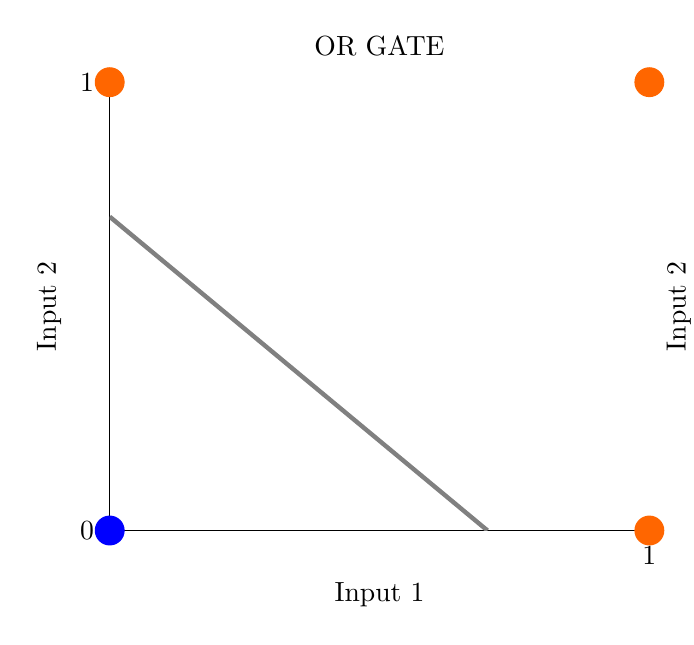
\begin{tikzpicture}
\definecolor{my_orange}{RGB}{255,102,0}
\pgfplotsset{soldot/.style={color=my_orange,only marks,mark=*,mark size=5.2,}}
\pgfplotsset{blue_soldot/.style={color=blue,only marks,mark=*,mark size=5.2,}}
\pgfplotsset{ignore zero/.style={%
#1ticklabel={\ifdim\tick pt=0pt \else\pgfmathprintnumber{\tick}\fi}
}}

\begin{axis}[
title = OR GATE,
axis lines = left,
xtick={0,1},
ytick={0,1},
xlabel = Input 1,
ylabel = Input 2,
axis line style={black},
every axis label/.append style ={black},
every tick label/.append style={black},
xmin=0,ymin=0,domain=0:1,ignore zero=x
]
%Below the red parabola is defined
\addplot [color=gray,ultra thick,domain=0:0.7]{ -x+0.7};
\addplot[blue_soldot] coordinates{(0,0)};
\addplot[soldot] coordinates{(0,1)};
\addplot[soldot] coordinates{(1,1)};
\addplot[soldot] coordinates{(1,0)};
\end{axis}

\begin{axis}[
title = XOR GATE,
axis lines = left,
xtick={0,1},
ytick={0,1},
xlabel = Input 1,
ylabel = Input 2,
axis line style={black},
every axis label/.append style ={black},
every tick label/.append style={black},
xmin=0,ymin=0,domain=0:1,ignore zero=x
]
\hspace{8cm}
%Below the red parabola is defined
\addplot [color=gray,ultra thick]{ -x+0.7};
\addplot [color=gray,ultra thick,domain=0.3:1]{ -x+1.3};
\addplot[blue_soldot] coordinates{(0,0)};
\addplot[soldot] coordinates{(0,1)};
\addplot[blue_soldot] coordinates{(1,1)};
\addplot[soldot] coordinates{(1,0)};
\end{axis}

\end{tikzpicture}


\caption{}
\label{fig:placeholder}
\end{figure}
% }}}
% tkiz two column {{{

\begin{figure}[h!]
\begin{tikzpicture}[>=stealth]

\tikzset{%
every neuron/.style={
circle,
draw,
minimum size=2cm
},
neuron missing/.style={
draw=none,
scale=4,
text height=0.333cm,
execute at begin node=\color{white}$\vdots$
},
}

% Number of Input Layer Node Circles to display
\foreach \m/\l [count=\y] in {1,missing, missing,2}
\node [every neuron/.try, neuron \m/.try] (input-\m) at (0,1.5-\y) {b = 0};

% Number of Hidden Layer Node Circles to display
\foreach \m [count=\y] in {1,missing, missing,2}
\node [every neuron/.try, neuron \m/.try ] (hidden-\m) at (3,1.5-\y) {b = -10};

% Number of Output Layer Node Circles to display
\foreach \m [count=\y] in {1}
\node [every neuron/.try, neuron \m/.try ] (output-\m) at (6,0-\y) {b= 30};

% Input layer arrow and labels
\foreach \l [count=\i] in {1,2}
\draw [<-] (input-\i) -- ++(-1,0) node [above, midway] {$x_\l$};

% Hidden layer 1 arrow and labels
%\foreach \l [count=\i] in {1,2} \node [above] at (hidden-\i.north) ;

% Output layer arrow and labels
%\foreach \l [count=\i] in {1} \draw [->] (output-\i) -- ++(1,0)
%node [above, right] {$Output$};

% Highlight Specific Weights and label them
%\draw [red,->] (input-1) -- node[auto] {$w=+20$} (hidden-1);
%\draw [red,->] (input-1) -- node[auto,left] {$w=-20$} (hidden-2);

%\draw [blue,->] (input-2) -- node[auto,end, right] {$w=+20$} (hidden-1);
%\draw [blue,->] (input-2) -- node[auto,end] {$w=-20$} (hidden-2);

%\draw [green,->] (hidden-1) -- node[auto,midway] {$w=+20$} (output-1);
%\draw [green,->] (hidden-2) -- node[auto] {$w=+20$} (output-1);

\end{tikzpicture}


\caption{}
\label{fig:placeholder}
\end{figure}
% }}}

% tkiz two column {{{

\begin{figure}[h!]
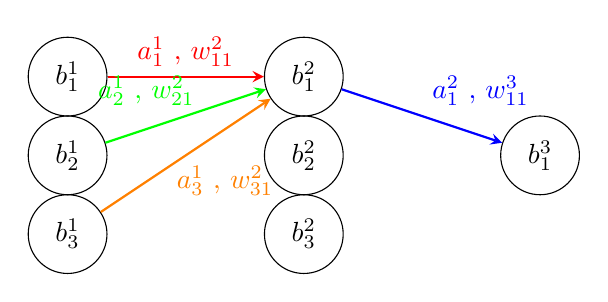
\begin{tikzpicture}[>=stealth]

\tikzset{%
every neuron/.style={
circle,
draw,
minimum size=1cm
},
neuron missing/.style={
draw=none,
scale=4,
text height=0.333cm,
execute at begin node=\color{white}$\vdots$
},
}

% Number of Input Layer Node Circles to display
\foreach \m/\l [count=\y] in {1,2,3}
\node [every neuron/.try, neuron \m/.try] (input-\m) at (0,2-\y) {$b_{\y}^{1}$};

% Number of Hidden Layer Node Circles to display
\foreach \m [count=\y] in {1,2,3}
\node [every neuron/.try, neuron \m/.try ] (hidden-\m) at (3,2-\y) {$b_{\y}^{2}$};

% Number of Output Layer Node Circles to display
\foreach \m [count=\y] in {1}
\node [every neuron/.try, neuron \m/.try ] (output-\m) at (6,1-\y) {$b_{\y}^{3}$};

% Input layer arrow and labels
%\foreach \l [count=\i] in {1,2,3}
%\draw [<-] (input-\i) -- ++(-1,0) node [above, midway] {$a_\l^{0}$};

% Hidden layer 1 arrow and labels
%\foreach \l [count=\i] in {1,2,3} \node [above] at (hidden-\i.north) {};

% Output layer arrow and labels
%\foreach \l [count=\i] in {1} \draw [->] (output-\i) -- ++(1,0)
%node [above, midway] {$a_\l^3$};

% Highlight Specific Weights and label them
\draw [red, thick, ->] (input-1) -- node[auto] {$a_{1}^{1}$ , $w_{11}^{2}$} (hidden-1);
\draw [green, thick, ->] (input-2) -- node[auto,above] {$a_{2}^{1}$ , $w_{21}^{2} \hspace{10mm}$} (hidden-1);
\draw [orange, thick, ->] (input-3) -- node[auto,below] {$\hspace{10mm} a_{3}^{1}$ , $w_{31}^{2}$} (hidden-1);
\draw [blue, thick, ->] (hidden-1) -- node[auto] {$a_{1}^{2}$ , $w_{11}^{3}$} (output-1);

% Labelling the layers
%\foreach \l [count=\x from 0] in {Input, Hidden, Output}
%\node [align=center, above] at (\x*3,2) {\l \\ layer};

\end{tikzpicture}


\caption{}
\label{fig:placeholder}
\end{figure}
% }}}
% till line 120 in neural nets and backprop





% pog {{{
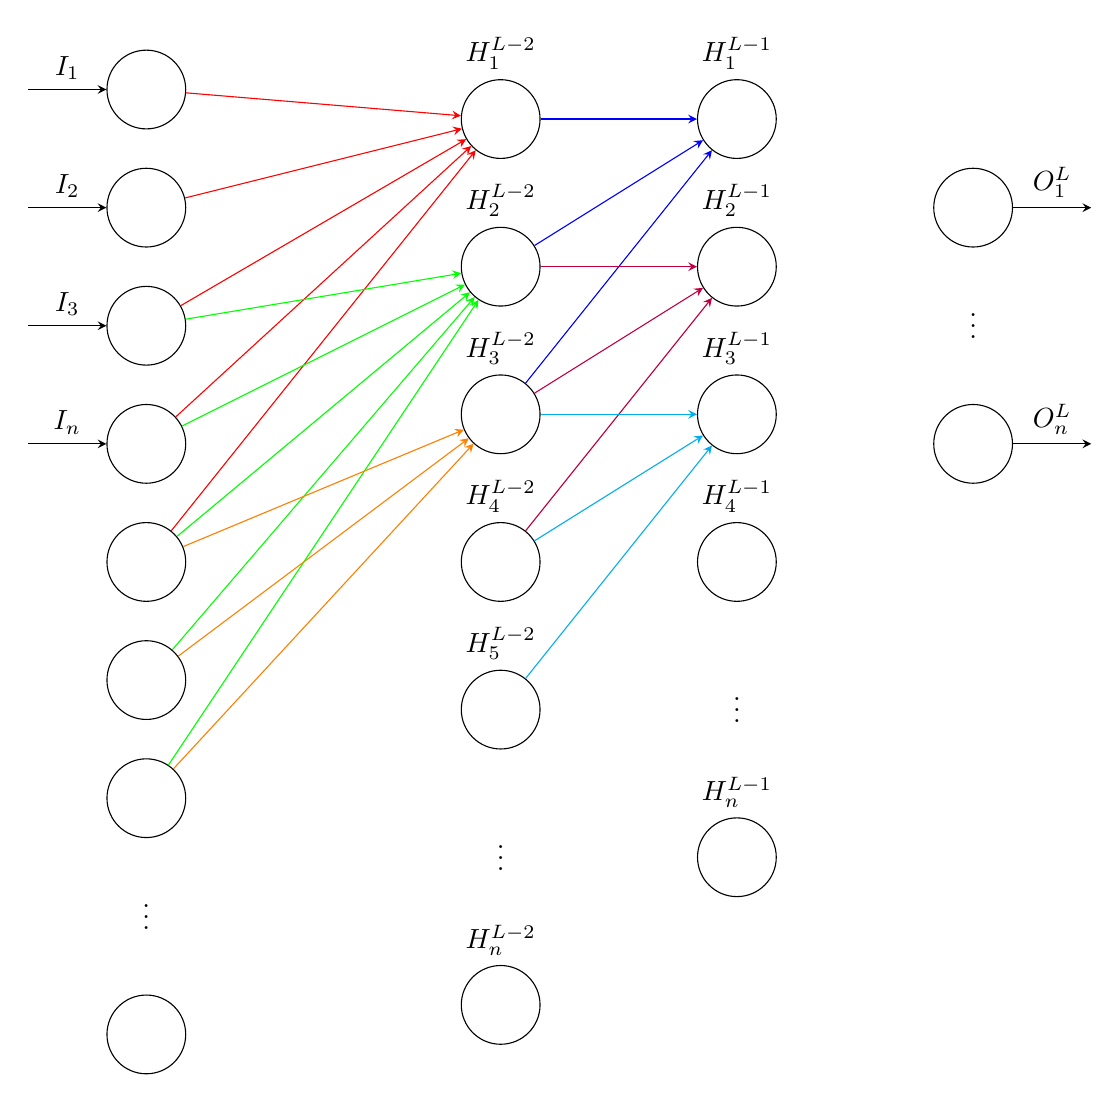
\begin{tikzpicture}[x=1.5cm, y=1.5cm, >=stealth,anchor = north west]


    
    \tikzset{%
    every neuron/.style={
        circle,
        draw,
        minimum size=1cm
        },
    neuron missing/.style={
        draw=none,
        %scale=2,
        text height=0.333cm,
        execute at begin node=\color{black}$\vdots$
        },
    }
    

    % Number of Input Layer Node Circles to display
    \foreach \m/\l [count=\y] in {1,2,3,4,5,6,7,missing,8}
    \node [every neuron/.try, neuron \m/.try] (input-\m) at (0,2.5-\y) {};
    
    % Number of Hidden Layer Node Circles to display
    \foreach \m [count=\y] in {1,2,3,4,5,missing,6}
    \node [every neuron/.try, neuron \m/.try ] (hidden-\m) at (3,2.5-\y*1.25) {};
    
    % Number of Hidden layer 2 Node Circles to display
    \foreach \m [count=\y] in {1,2,3,4,missing,5}
    \node [every neuron/.try, neuron \m/.try ] (hidden2-\m) at (5,2.5-\y*1.25) {};
    
    % Number of Output Layer Node Circles to display
    \foreach \m [count=\y] in {1,missing,2}
    \node [every neuron/.try, neuron \m/.try ] (output-\m) at (7,1.5-\y) {};
    
    % Input layer arrow and labels
    \foreach \l [count=\i] in {1,2,3,n}
    \draw [<-] (input-\i) -- ++(-1,0) node [above, midway] {$I_\l$};
    
    % Hidden layer 1 arrow and labels
    \foreach \l [count=\i] in {1,2,3,4,5,n} \node [above] at (hidden-\i.north) {$H_\l^{L-2}$};
    
    % Hidden layer 2 arrow and labels
    \foreach \l [count=\i] in {1,2,3,4,n} \node [above] at (hidden2-\i.north) {$H_\l^{L-1}$};
    
    % Output layer arrow and labels
    \foreach \l [count=\i] in {1,n} \draw [->] (output-\i) -- ++(1,0)
    node [above, midway] {$O_\l^L$};
    
   
    
    % Highlight Specific Weights and label them
    \draw [red,->] (input-1) -- node[auto] {} (hidden-1);
    \draw [red,->] (input-2) -- node[auto] {} (hidden-1);
    \draw [red,->] (input-3) -- node[auto] {} (hidden-1);
    \draw [red,->] (input-4) -- node[auto] {} (hidden-1);
    \draw [red,->] (input-5) -- node[auto] {} (hidden-1);
    
    \draw [green,->] (input-3) -- node[auto] {} (hidden-2);
    \draw [green,->] (input-4) -- node[auto] {} (hidden-2);
    \draw [green,->] (input-5) -- node[auto] {} (hidden-2);
    \draw [green,->] (input-6) -- node[auto] {} (hidden-2);
    \draw [green,->] (input-7) -- node[auto] {} (hidden-2);
   
    \draw [orange,->] (input-5) -- node[auto] {} (hidden-3);
    \draw [orange,->] (input-6) -- node[auto] {} (hidden-3);
    \draw [orange,->] (input-7) -- node[auto] {} (hidden-3);
    
    \draw [blue,->] (hidden-1) -- node[auto] {} (hidden2-1);
    \draw [blue,->] (hidden-2) -- node[auto] {} (hidden2-1);
    \draw [blue,->] (hidden-3) -- node[auto] {} (hidden2-1);
    
    \draw [purple,->] (hidden-2) -- node[auto] {} (hidden2-2);
    \draw [purple,->] (hidden-3) -- node[auto] {} (hidden2-2);
    \draw [purple,->] (hidden-4) -- node[auto] {} (hidden2-2);
    
    \draw [cyan,->] (hidden-3) -- node[auto] {} (hidden2-3);
    \draw [cyan,->] (hidden-4) -- node[auto] {} (hidden2-3);
    \draw [cyan,->] (hidden-5) -- node[auto] {} (hidden2-3);
    
\end{tikzpicture}

% }}}
\pagebreak

% champ {{{

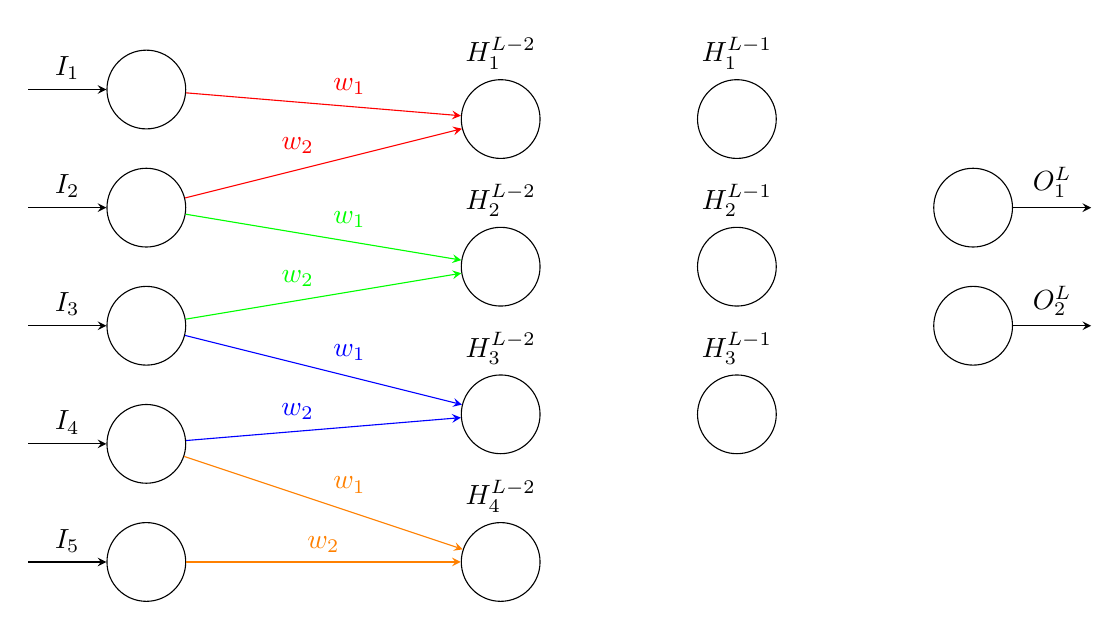
\begin{tikzpicture}[x=1.5cm, y=1.5cm, >=stealth,anchor = north west]


    
    \tikzset{%
    every neuron/.style={
        circle,
        draw,
        minimum size=1cm
        },
    neuron missing/.style={
        draw=none,
        %scale=2,
        text height=0.333cm,
        execute at begin node=\color{black}$\vdots$
        },
    }
    

    % Number of Input Layer Node Circles to display
    \foreach \m/\l [count=\y] in {1,2,3,4,5}
    \node [every neuron/.try, neuron \m/.try] (input-\m) at (0,2.5-\y) {};
    
    % Number of Hidden Layer Node Circles to display
    \foreach \m [count=\y] in {1,2,3,4}
    \node [every neuron/.try, neuron \m/.try ] (hidden-\m) at (3,2.5-\y*1.25) {};
    
    % Number of Hidden layer 2 Node Circles to display
    \foreach \m [count=\y] in {1,2,3}
    \node [every neuron/.try, neuron \m/.try ] (hidden2-\m) at (5,2.5-\y*1.25) {};
    
    % Number of Output Layer Node Circles to display
    \foreach \m [count=\y] in {1,2}
    \node [every neuron/.try, neuron \m/.try ] (output-\m) at (7,1.5-\y) {};
    
    % Input layer arrow and labels
    \foreach \l [count=\i] in {1,2,3,4,5}
    \draw [<-] (input-\i) -- ++(-1,0) node [above, midway] {$I_\l$};
    
    % Hidden layer 1 labels
    \foreach \l [count=\i] in {1,2,3,4} \node [above] at (hidden-\i.north) {$H_\l^{L-2}$};
    
    % Hidden layer 2 labels
    \foreach \l [count=\i] in {1,2,3} \node [above] at (hidden2-\i.north) {$H_\l^{L-1}$};
    
    % Output layer labels
    \foreach \l [count=\i] in {1,2} \draw [->] (output-\i) -- ++(1,0)
    node [above, midway] {$O_\l^L$};
    
   
    
    % Highlight Specific Weights and label them
    \draw [red,->] (input-1) -- node[auto] {$w_1$} (hidden-1);
    \draw [red,->] (input-2) -- node[auto] {$w_2$} (hidden-1);
    
    \draw [green,->] (input-2) -- node[auto] {$w_1$} (hidden-2);
    \draw [green,->] (input-3) -- node[auto] {$w_2$} (hidden-2);
    
    \draw [blue,->] (input-3) -- node[auto] {$w_1$} (hidden-3);
    \draw [blue,->] (input-4) -- node[auto] {$w_2$} (hidden-3);
   
    \draw [orange,->] (input-4) -- node[auto] {$w_1$} (hidden-4);
    \draw [orange,->] (input-5) -- node[auto] {$w_2$} (hidden-4);
    
    
\end{tikzpicture}


% }}}

% ion {{{
\begin{tikzpicture}[x=1.5cm, y=1.5cm, >=stealth,anchor = north west]


    
    \tikzset{%
    every neuron/.style={
        circle,
        draw,
        minimum size=1cm
        },
    neuron missing/.style={
        draw=none,
        %scale=2,
        text height=0.333cm,
        execute at begin node=\color{black}$\vdots$
        },
    }
    
    % Number of Input Layer Node Circles to display
    \foreach \m/\l [count=\y] in {1,2,3,4,5,6,7,8}
    \node [every neuron/.try, neuron \m/.try] (input-\m) at (0,2.5-\y) {};
    
    % Number of Hidden Layer Node Circles to display
    \foreach \m [count=\y] in {1,2,3,4}
    \node [every neuron/.try, neuron \m/.try ] (hidden-\m) at (3,2.5-\y*1.25) {};
    
   
    
    % Number of Output Layer Node Circles to display
    \foreach \m [count=\y] in {1,2}
    \node [every neuron/.try, neuron \m/.try ] (output-\m) at (5,1.5-\y) {};
    
    
    \draw [<-] (input-1) -- ++(-2,0) node [above, midway] {$PADDING$};
    \draw [<-] (input-8) -- ++(-2,0) node [above, midway] {$PADDING$};
    
    % Hidden layer 1 labels
    \foreach \l [count=\i] in {1,2,3,4} \node [above] at (hidden-\i.north) {$H_\l$};
    
    
    % Output layer labels
    \foreach \l [count=\i] in {1,2} \draw [->] (output-\i) -- ++(1,0)
    node [above, midway] {$O_\l$};
    
   
    
    % Highlight Specific Weights and label them
    \draw [black,->] (input-1) -- node[auto] {} (hidden-1);
    \draw [black,->] (input-2) -- node[auto] {} (hidden-1);
    
    \draw [black,->] (input-3) -- node[auto] {} (hidden-2);
    \draw [black,->] (input-4) -- node[auto] {} (hidden-2);
    
    \draw [black,->] (input-5) -- node[auto] {} (hidden-3);
    \draw [black,->] (input-6) -- node[auto] {} (hidden-3);
    
    \draw [black,->] (input-7) -- node[auto] {} (hidden-4);
    \draw [black,->] (input-8) -- node[auto] {} (hidden-4);
    
    
\end{tikzpicture}


% }}}

%  {{{
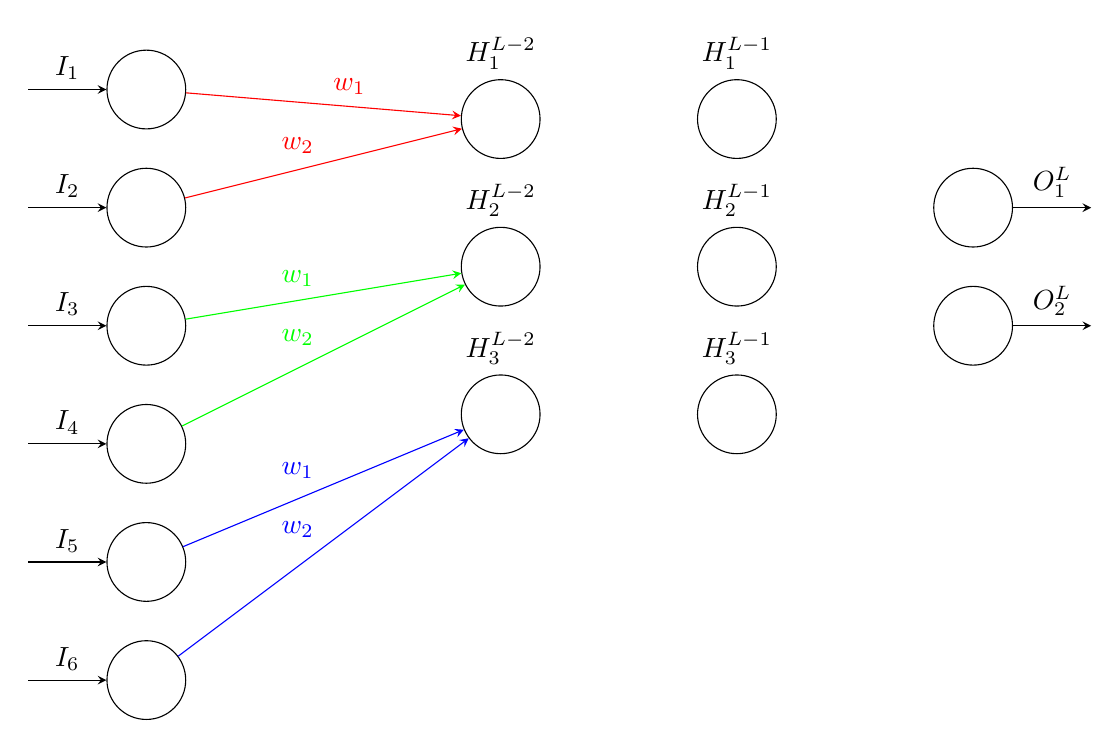
\begin{tikzpicture}[x=1.5cm, y=1.5cm, >=stealth,anchor = north west]


    
    \tikzset{%
    every neuron/.style={
        circle,
        draw,
        minimum size=1cm
        },
    neuron missing/.style={
        draw=none,
        %scale=2,
        text height=0.333cm,
        execute at begin node=\color{black}$\vdots$
        },
    }
    
    % Number of Input Layer Node Circles to display
    \foreach \m/\l [count=\y] in {1,2,3,4,5,6}
    \node [every neuron/.try, neuron \m/.try] (input-\m) at (0,2.5-\y) {};
    
    % Number of Hidden Layer Node Circles to display
    \foreach \m [count=\y] in {1,2,3}
    \node [every neuron/.try, neuron \m/.try ] (hidden-\m) at (3,2.5-\y*1.25) {};
    
    % Number of Hidden layer 2 Node Circles to display
    \foreach \m [count=\y] in {1,2,3}
    \node [every neuron/.try, neuron \m/.try ] (hidden2-\m) at (5,2.5-\y*1.25) {};
    
    % Number of Output Layer Node Circles to display
    \foreach \m [count=\y] in {1,2}
    \node [every neuron/.try, neuron \m/.try ] (output-\m) at (7,1.5-\y) {};
    
    % Input layer arrow and labels
    \foreach \l [count=\i] in {1,2,3,4,5,6}
    \draw [<-] (input-\i) -- ++(-1,0) node [above, midway] {$I_\l$};
    
    % Hidden layer 1 labels
    \foreach \l [count=\i] in {1,2,3} \node [above] at (hidden-\i.north) {$H_\l^{L-2}$};
    
    % Hidden layer 2 labels
    \foreach \l [count=\i] in {1,2,3} \node [above] at (hidden2-\i.north) {$H_\l^{L-1}$};
    
    % Output layer labels
    \foreach \l [count=\i] in {1,2} \draw [->] (output-\i) -- ++(1,0)
    node [above, midway] {$O_\l^L$};
    
   
    
    % Highlight Specific Weights and label them
    \draw [red,->] (input-1) -- node[auto] {$w_1$} (hidden-1);
    \draw [red,->] (input-2) -- node[auto] {$w_2$} (hidden-1);
    
    \draw [green,->] (input-3) -- node[auto] {$w_1$} (hidden-2);
    \draw [green,->] (input-4) -- node[auto] {$w_2$} (hidden-2);
    
    \draw [blue,->] (input-5) -- node[auto] {$w_1$} (hidden-3);
    \draw [blue,->] (input-6) -- node[auto] {$w_2$} (hidden-3);
    
    
\end{tikzpicture}



% }}}

%  {{{
\begin{tikzpicture}[x=1.5cm, y=1.5cm, >=stealth,anchor = north west]


    
    \tikzset{%
    every neuron/.style={
        circle,
        draw,
        minimum size=1cm
        },
    neuron missing/.style={
        draw=none,
        %scale=2,
        text height=0.333cm,
        execute at begin node=\color{black}$\vdots$
        },
    }
    
    \tikzset{%
    every neuron2/.style={
        circle,
        draw,
        minimum size=1cm,
        fill=gray1
        },
    neuron missing/.style={
        draw=none,
        %scale=2,
        text height=0.333cm,
        execute at begin node=\color{black}$\vdots$
        },
    }
    
    

    % Number of Input Layer Node Circles to display
    \foreach \m/\l [count=\y] in {1,2,3,4,5}
    \node [every neuron/.try, neuron \m/.try] (input-\m) at (0,2.5-\y) {};
    
    % Number of Hidden Layer Node Circles to display
    \foreach \m [count=\y] in {1,2,3,4}
    \node [every neuron/.try, neuron \m/.try ] (hidden-\m) at (3,2.5-\y*1.25) {};
   
   
   % Display number of filters
    \foreach \m [count=\y] in {1,2,3,4}
    \node [every neuron2/.try, neuron \m/.try ] (hidden2-\m) at (3.25,2.5-\y*1.4) {};
    
    \foreach \m [count=\y] in {1,2,3,4}
    \node [every neuron3/.try, neuron \m/.try ] (hidden3-\m) at (3.5,2.5-\y*1.35) {};
    
    \foreach \m [count=\y] in {1,2,3,4}
    \node [every neuron4/.try, neuron \m/.try ] (hidden4-\m) at (3.75,2.5-\y*1.4) {};
    
    % Number of Output Layer Node Circles to display
    \foreach \m [count=\y] in {1,2}
    \node [every neuron/.try, neuron \m/.try ] (output-\m) at (5,1.5-\y) {};
    
    % Input layer arrow and labels
    \foreach \l [count=\i] in {1,2,3,4,5}
    \draw [<-] (input-\i) -- ++(-1,0) node [above, midway] {$I_\l$};
        
    % Output layer labels
    \foreach \l [count=\i] in {1,2} \draw [->] (output-\i) -- ++(1,0)
    node [above, midway] {$O_\l^L$};
    
   
    
    % Highlight Specific Weights and label them
    \draw [red,->] (input-1) -- node[auto] {} (hidden-1);
    \draw [red,->] (input-2) -- node[auto] {}(hidden-1);
    
    \draw [green,->] (input-2) -- node[auto] {}(hidden-2);
    \draw [green,->] (input-3) -- node[auto] {}(hidden-2);
    
    \draw [blue,->] (input-3) -- node[auto] {}(hidden-3);
    \draw [blue,->] (input-4) -- node[auto]{} (hidden-3);
   
    \draw [orange,->] (input-4) -- node[auto] {} (hidden-4);
    \draw [orange,->] (input-5) -- node[auto] {} (hidden-4);
    
    % Filters
    
    \draw [gray,->] (input-1) -- node[auto] {} (hidden2-1);
    \draw [gray,->] (input-2) -- node[auto] {}(hidden2-1);
    
    \draw [black,->] (input-2) -- node[auto] {}(hidden2-2);
    \draw [black,->] (input-3) -- node[auto] {}(hidden2-2);
    
    \draw [cyan,->] (input-3) -- node[auto] {}(hidden2-3);
    \draw [cyan,->] (input-4) -- node[auto]{} (hidden2-3);
   
    \draw [magenta,->] (input-4) -- node[auto] {} (hidden2-4);
    \draw [magenta,->] (input-5) -- node[auto] {} (hidden2-4);
    
\end{tikzpicture}

% }}}
%  {{{
\begin{tikzpicture}[x=1.5cm, y=1.5cm, >=stealth,anchor = north west]


    
    \tikzset{%
    every neuron/.style={
        circle,
        draw,
        minimum size=1cm
        },
    neuron missing/.style={
        draw=none,
        %scale=2,
        text height=0.333cm,
        execute at begin node=\color{black}$\vdots$
        },
    }
    
    \tikzset{%
    every neuron2/.style={
        circle,
        draw,
        minimum size=1cm,
        fill=gray1
        },
    neuron missing/.style={
        draw=none,
        %scale=2,
        text height=0.333cm,
        execute at begin node=\color{black}$\vdots$
        },
    }
    
    

    % Number of Input Layer Node Circles to display
    \foreach \m/\l [count=\y] in {1,2,3,4,5}
    \node [every neuron/.try, neuron \m/.try] (input-\m) at (0,2.5-\y) {};
    
    % Number of Hidden Layer Node Circles to display
    \foreach \m [count=\y] in {1,2,3,4}
    \node [every neuron/.try, neuron \m/.try ] (hidden-\m) at (3,2.5-\y*1.25) {};
   
   
   % Display number of filters
    \foreach \m [count=\y] in {1,2,3,4}
    \node [every neuron2/.try, neuron \m/.try ] (hidden2-\m) at (3.25,2.5-\y*1.4) {};
    
    \foreach \m [count=\y] in {1,2,3,4}
    \node [every neuron3/.try, neuron \m/.try ] (hidden3-\m) at (3.5,2.5-\y*1.35) {};
    
    \foreach \m [count=\y] in {1,2,3,4}
    \node [every neuron4/.try, neuron \m/.try ] (hidden4-\m) at (3.75,2.5-\y*1.4) {};
    
    % Number of Output Layer Node Circles to display
    \foreach \m [count=\y] in {1,2}
    \node [every neuron/.try, neuron \m/.try ] (output-\m) at (5,1.5-\y) {};
    
    % Input layer arrow and labels
    \foreach \l [count=\i] in {1,2,3,4,5}
    \draw [<-] (input-\i) -- ++(-1,0) node [above, midway] {$I_\l$};
        
    % Output layer labels
    \foreach \l [count=\i] in {1,2} \draw [->] (output-\i) -- ++(1,0)
    node [above, midway] {$O_\l^L$};
    
   
    
    % Highlight Specific Weights and label them
    \draw [red,->] (input-1) -- node[auto] {} (hidden-1);
    \draw [red,->] (input-2) -- node[auto] {}(hidden-1);
    
    \draw [green,->] (input-2) -- node[auto] {}(hidden-2);
    \draw [green,->] (input-3) -- node[auto] {}(hidden-2);
    
    \draw [blue,->] (input-3) -- node[auto] {}(hidden-3);
    \draw [blue,->] (input-4) -- node[auto]{} (hidden-3);
   
    \draw [orange,->] (input-4) -- node[auto] {} (hidden-4);
    \draw [orange,->] (input-5) -- node[auto] {} (hidden-4);
    
    % Filters
    
    \draw [gray,->] (input-1) -- node[auto] {} (hidden2-1);
    \draw [gray,->] (input-2) -- node[auto] {}(hidden2-1);
    
    \draw [black,->] (input-2) -- node[auto] {}(hidden2-2);
    \draw [black,->] (input-3) -- node[auto] {}(hidden2-2);
    
    \draw [cyan,->] (input-3) -- node[auto] {}(hidden2-3);
    \draw [cyan,->] (input-4) -- node[auto]{} (hidden2-3);
   
    \draw [magenta,->] (input-4) -- node[auto] {} (hidden2-4);
    \draw [magenta,->] (input-5) -- node[auto] {} (hidden2-4);
    
\end{tikzpicture}


% }}}

%  {{{
\begin{tikzpicture}[x=1.5cm, y=1.5cm, >=stealth,anchor = north west]


    
    \tikzset{%
    every neuron/.style={
        circle,
        draw,
        minimum size=1cm
        },
    neuron missing/.style={
        draw=none,
        %scale=2,
        text height=0.333cm,
        execute at begin node=\color{black}$\vdots$
        },
    }
    
    \tikzset{%
    every neuron2/.style={
        circle,
        draw,
        minimum size=1cm,
        fill=gray1
        },
    neuron missing/.style={
        draw=none,
        %scale=2,
        text height=0.333cm,
        execute at begin node=\color{black}$\vdots$
        },
    }
    
    \tikzset{%
    every neuron3/.style={
        circle,
        draw,
        minimum size=1cm,
        fill=gray2
        },
    neuron missing/.style={
        draw=none,
        %scale=2,
        text height=0.333cm,
        execute at begin node=\color{black}$\vdots$
        },
    }
    
    \tikzset{%
    every neuron4/.style={
        circle,
        draw,
        minimum size=1cm,
        fill=gray3
        },
    neuron missing/.style={
        draw=none,
        %scale=2,
        text height=0.333cm,
        execute at begin node=\color{black}$\vdots$
        },
    }
    

    % Number of Input Layer Node Circles to display
    \foreach \m/\l [count=\y] in {1,2,3,4,5}
    \node [every neuron/.try, neuron \m/.try] (input-\m) at (0,2.5-\y) {};
    
    % Number of Hidden Layer Node Circles to display
    \foreach \m [count=\y] in {1,2,3,4}
    \node [every neuron/.try, neuron \m/.try ] (hidden-\m) at (3,2.5-\y*1.25) {};
   
   
   % Display number of filters
    \foreach \m [count=\y] in {1,2,3,4}
    \node [every neuron2/.try, neuron \m/.try ] (hidden2-\m) at (3.25,2.5-\y*1.3) {};
    
    \foreach \m [count=\y] in {1,2,3,4}
    \node [every neuron3/.try, neuron \m/.try ] (hidden3-\m) at (3.5,2.5-\y*1.35) {};
    
    \foreach \m [count=\y] in {1,2,3,4}
    \node [every neuron4/.try, neuron \m/.try ] (hidden4-\m) at (3.75,2.5-\y*1.4) {};
    
    % Number of Output Layer Node Circles to display
    \foreach \m [count=\y] in {1,2}
    \node [every neuron/.try, neuron \m/.try ] (output-\m) at (5,1.5-\y) {};
    
    % Input layer arrow and labels
    \foreach \l [count=\i] in {1,2,3,4,5}
    \draw [<-] (input-\i) -- ++(-1,0) node [above, midway] {$I_\l$};
        
    % Output layer labels
    \foreach \l [count=\i] in {1,2} \draw [->] (output-\i) -- ++(1,0)
    node [above, midway] {$O_\l^L$};
    
   
    
    % Highlight Specific Weights and label them
    \draw [black,->] (input-1) -- node[auto] {} (hidden-1);
    \draw [black,->] (input-2) -- node[auto] {}(hidden-1);
    
    \draw [black,->] (input-2) -- node[auto] {}(hidden-2);
    \draw [black,->] (input-3) -- node[auto] {}(hidden-2);
    
    \draw [black,->] (input-3) -- node[auto] {}(hidden-3);
    \draw [black,->] (input-4) -- node[auto]{} (hidden-3);
   
    \draw [black,->] (input-4) -- node[auto] {} (hidden-4);
    \draw [black,->] (input-5) -- node[auto] {} (hidden-4);
    
    %filter1
    
     \draw [black,->] (input-1) -- node[auto] {} (hidden2-1);
    \draw [black,->] (input-2) -- node[auto] {}(hidden2-1);
    
    \draw [black,->] (input-2) -- node[auto] {}(hidden2-2);
    \draw [black,->] (input-3) -- node[auto] {}(hidden2-2);
    
    \draw [black,->] (input-3) -- node[auto] {}(hidden2-3);
    \draw [black,->] (input-4) -- node[auto]{} (hidden2-3);
   
    \draw [black,->] (input-4) -- node[auto] {} (hidden2-4);
    \draw [black,->] (input-5) -- node[auto] {} (hidden2-4);
    
    %filter2
     \draw [black,->] (input-1) -- node[auto] {} (hidden3-1);
    \draw [black,->] (input-2) -- node[auto] {}(hidden3-1);
    
    \draw [black,->] (input-2) -- node[auto] {}(hidden3-2);
    \draw [black,->] (input-3) -- node[auto] {}(hidden3-2);
    
    \draw [black,->] (input-3) -- node[auto] {}(hidden3-3);
    \draw [black,->] (input-4) -- node[auto]{} (hidden3-3);
   
    \draw [black,->] (input-4) -- node[auto] {} (hidden3-4);
    \draw [black,->] (input-5) -- node[auto] {} (hidden3-4);
    
    %filter3
     \draw [black,->] (input-1) -- node[auto] {} (hidden4-1);
    \draw [black,->] (input-2) -- node[auto] {}(hidden4-1);
    
    \draw [black,->] (input-2) -- node[auto] {}(hidden4-2);
    \draw [black,->] (input-3) -- node[auto] {}(hidden4-2);
    
    \draw [black,->] (input-3) -- node[auto] {}(hidden4-3);
    \draw [black,->] (input-4) -- node[auto]{} (hidden4-3);
   
    \draw [black,->] (input-4) -- node[auto] {} (hidden4-4);
    \draw [black,->] (input-5) -- node[auto] {} (hidden4-4);
    
    
\end{tikzpicture}

% }}}

% ----------------------------------------------------------------------------- 
\end{document}
% =============================================================================
% - EOF - EOF - EOF - EOF - EOF - EOF - EOF - EOF - EOF - EOF - EOF - EOF -
% =============================================================================

